
\chapter{Introduction\label{ch:intro}}

% Talk about the increasing use of quadcopters for a variety of uses.
In recent years, research using small-scale Unmanned Aerial Vehicles (UAVs) has increased rapidly. Multi-rotor aircraft, such as quadcopters (also known as quadrotors), have proven to be powerful platforms for applications in a variety of fields, from aerial photography to search and rescue~\cite{Irschara, Gupte}. Once prohibitively expensive for many applications, multi-rotor aircraft have decreased substantially in price, ranging from a few hundred dollars to several thousand dollars. Additionally, on-board control systems have greatly added to the stability and ease of control of these aircraft, with many quadcopters using pre-programmed routines for difficult procedures such as takeoff and landing.


%Slightly repetitive. Also should this be in the related work section? What is the best way to split this up?
Although quadcopters have seen interest from the military and hobbyists for quite some time, these recent developments in price and stability have resulted in a large increase of research using quadcopters. In 2010, a French electronics company, Parrot, released the AR.Drone, a quadcopter intended for consumers. Unlike most other quadcopters, which are sold in unassembled kits targeted to experienced hobbyists or researchers, the AR.Drone was designed to be ready-to-fly right out of the box by an inexperienced pilot. Although affordable and easy to use, these quadcopters are far from just toys. Equipped with an array sensors and multiple cameras, the AR.Drone and other consumer-grade vehicles have been used by research groups to explore autonomous flight with a low barrier of entry, both in cost and complexity.

With the democratization of this technology, quadcopters can be used to be solved problems where cost and complexity for such a solution were once prohibitive.

\section{Motivation}

For applications ranging from developing video games to preserving archaeological artifacts, capturing 3D models of real-world objects has become an increasingly important task. %Talk more about why 3D is important 

While there are currently several different methods for capturing these models, each of these methods has associated limitations and drawbacks.


\section{Current Acquisition Methods}

\subsection{Manual Model Creation}
The most common method of model acquisition is using a trained modeler to manually produce a 3D model using reference imagery and measurements. Models are tediously crafted in CAD software in a process similar to sculpting. While this technique is used extensively in video games and films, it is typically too time consuming and expensive for many applications such as archeology.

\subsection{Laser Scanners}
Laser rangefinder technology is the ``gold standard'' of 3D model acquisition in terms of precision. Modern scanners are able to produce models with sub-millimeter precision, which make them a great choice for detailed digitization of statues. Combined with high-resolution photograph texture-mapping, very few techniques can match the precision and quality of these scans. The Digital Michelangelo Project showed the power and precision of laser scanners by scanning several different statues, including Michelangelo's David, to 1/4mm accuracy~\cite{Levoy}.

\begin{figure}
\centering
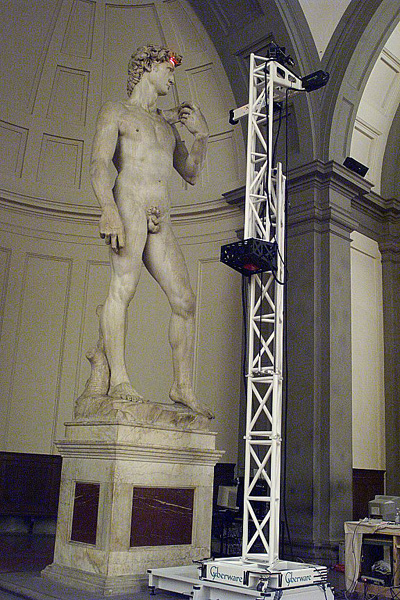
\includegraphics[height=200px]{../images/david_scan.jpg}
\caption{Laser scanner rig used by the Digital Michelangelo Project~\cite{Levoy}.}
\end{figure}

However, laser scanners do have several drawbacks. The equipment is extremely expensive, bulky, and fragile. The Michelangelo Project had to transport over 4 tons of equipment to Italy in order to produce their scans. Additionally, laser scans involve immense setup and can take many hours. The model of David took over a thousand man-hours to scan and even more than that in post processing~\cite{Levoy}.

\subsection{Microsoft Kinect}

Several groups have researched using the Microsoft Kinect for model acquisition. As the Kinect produces an RGB image with depth information, imagery gathered from multiple angles can be used to create a 3D model. While this has been found to be useful in scanning small to medium size objects, including people, the Kinect has several limitations. First of all, the depth range is rather short, on the order of a couple meters. Additionally, because the depth is partially determined using an infrared pattern, the Kinect does not work in locations with a large amount of background infrared light, such as outdoors.

\subsection{Multi-View Stereo}
Multi-view stereo uses a collection of 2D images to reconstruct a 3D object. By viewing a single object from hundreds of different camera positions, it is possible to infer depth information and generate a 3D model. Although this technique originally required precisely known camera coordinates, recent algorithms can produce a 3D model from an unordered collection of images with unknown camera positions, assuming that there is sufficient coverage. Existing software packages such as Bundler and Agisoft Photoscan can produce high-quality 3D reconstructions using these unordered image collections~\cite{bundler, Agisoft}.

The ability to use a collection of images without precise camera position information means that these 3D objects can be modeled substantially faster than with a laser scanner. For a smaller object, it is a relatively simple process to take pictures of the object from many different angles. However, for a larger object, such as a statue or building, the task of gathering imagery becomes substantially more difficult.

\begin{figure}
\centering
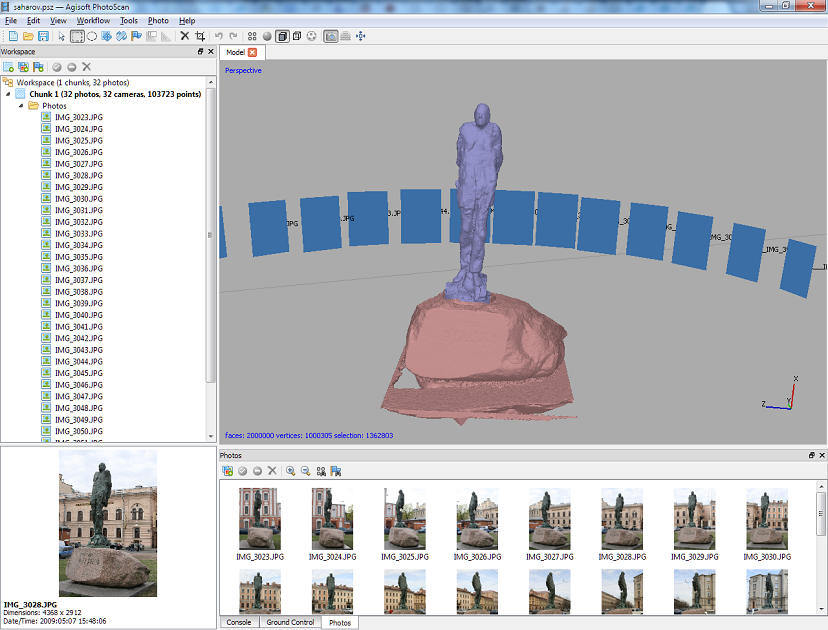
\includegraphics[height=200px]{../images/photoscan.png}
\caption{3D model of a statue generated by Agisoft Photoscan~\cite{Agisoft}.}
\end{figure}


\section{Problem Definition}
We look to create a system for capturing imagery of large objects for use in multi-view stereo software. There are several desirable attributes of such a system:

\begin{enumerate}
\item
\textbf{Low Cost}

The system should be low cost, making it accessible to as many users as possible.

\item
\textbf{Easy to Use}

The system should be able to be deployed by users with minimal training and setup. Additionally, the hardware should be off-the-shelf and easily attainable.

\item
\textbf{Complete Coverage}

The system must be able to capture images from a wide variety of positions, completely covering every part of the target object.

\item
\textbf{High Quality Imagery}

The system must produce sufficiently high resolution, non-distorted images for use in multi-view stereo software.

\end{enumerate}

\section{Proposed Solution}

We propose using low-cost autonomous quadcopters to gather the imagery needed for use in multi-view stereo software. By flying a quadcopter with a mounted camera around the target object, imagery can be gathered quickly from many viewing angles. Using quadcopters has many advantages:

\begin{figure}
\centering
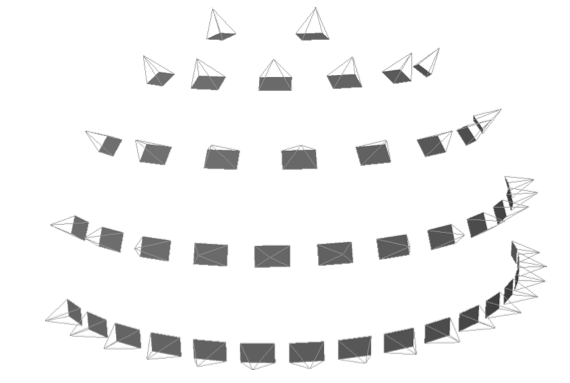
\includegraphics[width=200px]{../images/camera_network.png}
\caption{Example of desired camera positions for use in multi-view stereo~\cite{Irschara}.}
\end{figure}

\begin{enumerate}
\item
Quadcopters can capture images from positions unreachable by ground-based cameras.

\item
By methodically flying around the target object at different altitudes, complete coverage of the target object can be achieved.

\item
The imagery can be captured very quickly, on the order of a few minutes.

\item
Quadcopters are small, portable, and easily deployable.


\end{enumerate}

\section{Solution Components}

In order to implement such a solution, there are two main components which must be created. First, a localization algorithm is needed to produce position and orientation estimates of the quadcopter in the global frame. Then, a controller is needed to produce the control inputs for the quadcopter to move along a desired path. This thesis focuses on the design, implementation, and testing of the localization component, while the thesis of Sarah Tang in the Mechanical and Aerospace Engineering Department addresses the controller component of this system~\cite{Tang}.






